\documentclass{beamer}
\usepackage{lmodern}
\usepackage{multicol}
%\usepackage{graphicx}
%\usepackage{media9}
%\usepackage{tikz}
%\usepackage{multimedia}
\usepackage[3D]{movie15}


%\usetheme{Madrid}
\usetheme[progressbar=frametitle]{metropolis}
\setbeamertemplate{frame numbering}[fraction]
\useoutertheme{metropolis}
\useinnertheme{metropolis}
\usefonttheme{metropolis}
\usecolortheme{spruce}
\setbeamercolor{background canvas}{bg=white}

\definecolor{mygreen}{rgb}{0.125,0.5,0.25}
\usecolortheme[named=mygreen]{structure}
%\definecolor{azure(colorwheel)}{rgb}{0.0, 0.5, 1.0}
%\usecolortheme[named=azure(colorwheel)]{structure}




\title[Motion Planning for Quadrotors]{Trajectory Generation and Control for Quadrotors}
\author{Sandesh Thapa}
\institute[OSU-MAE]{Department of Mechanical and Aerospace Engineering \\ Oklahoma State University}
\date{}


\begin{document}
\metroset{block=fill}

\begin{frame}
\titlepage

\end{frame}

\begin{frame}[t]{Dynamic Model}\vspace{4pt}

\begin{columns}[onlytextwidth]
\column{0.5\textwidth}
\begin{figure}[h!]
\centering
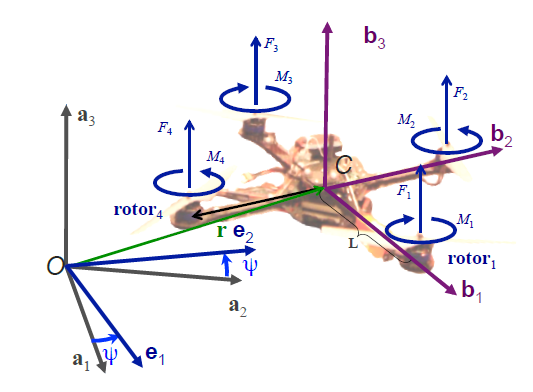
\includegraphics[scale=0.2]{images/Quadmodel.png}
\caption{Quadrotor model with the body-fixed and inertial reference frames.}
\label{Quadmodel}
\end{figure}
\column{0.5\textwidth}
\begin{enumerate}[A]
 \only<1->{
\item first}
\only<2->{
\item second}
\end{enumerate}

\end{columns}


\end{frame}



\begin{frame}[t]{Differential Flatness}\vspace{4pt}
\begin{block}{Definition}
blaaaaa
\end{block}
\end{frame}

\begin{frame}[t]{Robot Controller}\vspace{4pt}
xxx
\end{frame}

\begin{frame}[t]{Robot Controller}\vspace{4pt}
xxx
\end{frame}


\begin{frame}[t]{Minimum Snap Trajectory Generation}\vspace{4pt}
xxx
\end{frame}

%\begin{frame}{Test}
%      \begin{tikzpicture}[remember picture,overlay]
%         \node[anchor=south west, inner sep=0pt] at (current page.south west) {%
%           \includemedia[
%             addresource=TrajSim.avi,
%             activate=pageopen,transparent,
%             flashvars={source=TrajSim.avi},
%             width=0.5\paperwidth,height=0.5\paperheight
%           ]{}{VPlayer.swf}%
%         };
%      \end{tikzpicture}
%\end{frame}

%\begin{frame}
%\frametitle{Title}
%\movie[width=9cm,height=7cm, poster]{}{TrajSim.avi}
%\end{frame}

\begin{frame}{This is a movie showing a rotating wave}
\begin{picture}(320,300)
\put(0,80){\includemovie[poster, text={\small(Loading TrajSim.avi)}]{9cm}{6cm}{TrajSim.avi}}
\put(90,260){Rotating sine}
\end{picture}
\end{frame}
%
%\begin{frame}{}
%\begin{picture}(320,260)
%\put(-20,-30){\includegraphics[width=12.4cm]{TrajSim.avi}}
%\put(-19.8,244.4){\Large \bf This is a movie showing a rotating wave}
%\end{picture}
%\end{frame}

%\begin{frame}{embedded files}
%\includemedia[
%  width=0.4\linewidth,
%  totalheight=0.225\linewidth,
%  activate=pageopen,
%  passcontext,  %show VPlayer's right-click menu
%  addresource=TrajSim.avi,
%  flashvars={
%    %important: same path as in `addresource'
%    source=TrajSim.avi
%  }
%]{\fbox{Click!}}{VPlayer.swf}
%
%\end{frame}

\begin{frame}
%\begin{block}
\includemovie[autoplay,repeat]{4cm}{3cm}{TrajSim.avi}
%\end{block}
\end{frame}

\end{document}